% Options for packages loaded elsewhere
\PassOptionsToPackage{unicode}{hyperref}
\PassOptionsToPackage{hyphens}{url}
%
\documentclass[
  11pt,
]{article}
\usepackage{amsmath,amssymb}
\usepackage{iftex}
\ifPDFTeX
  \usepackage[T1]{fontenc}
  \usepackage[utf8]{inputenc}
  \usepackage{textcomp} % provide euro and other symbols
\else % if luatex or xetex
  \usepackage{unicode-math} % this also loads fontspec
  \defaultfontfeatures{Scale=MatchLowercase}
  \defaultfontfeatures[\rmfamily]{Ligatures=TeX,Scale=1}
\fi
\usepackage{lmodern}
\ifPDFTeX\else
  % xetex/luatex font selection
\fi
% Use upquote if available, for straight quotes in verbatim environments
\IfFileExists{upquote.sty}{\usepackage{upquote}}{}
\IfFileExists{microtype.sty}{% use microtype if available
  \usepackage[]{microtype}
  \UseMicrotypeSet[protrusion]{basicmath} % disable protrusion for tt fonts
}{}
\makeatletter
\@ifundefined{KOMAClassName}{% if non-KOMA class
  \IfFileExists{parskip.sty}{%
    \usepackage{parskip}
  }{% else
    \setlength{\parindent}{0pt}
    \setlength{\parskip}{6pt plus 2pt minus 1pt}}
}{% if KOMA class
  \KOMAoptions{parskip=half}}
\makeatother
\usepackage{xcolor}
\usepackage[margin=1in]{geometry}
\usepackage{color}
\usepackage{fancyvrb}
\newcommand{\VerbBar}{|}
\newcommand{\VERB}{\Verb[commandchars=\\\{\}]}
\DefineVerbatimEnvironment{Highlighting}{Verbatim}{commandchars=\\\{\}}
% Add ',fontsize=\small' for more characters per line
\usepackage{framed}
\definecolor{shadecolor}{RGB}{248,248,248}
\newenvironment{Shaded}{\begin{snugshade}}{\end{snugshade}}
\newcommand{\AlertTok}[1]{\textcolor[rgb]{0.94,0.16,0.16}{#1}}
\newcommand{\AnnotationTok}[1]{\textcolor[rgb]{0.56,0.35,0.01}{\textbf{\textit{#1}}}}
\newcommand{\AttributeTok}[1]{\textcolor[rgb]{0.13,0.29,0.53}{#1}}
\newcommand{\BaseNTok}[1]{\textcolor[rgb]{0.00,0.00,0.81}{#1}}
\newcommand{\BuiltInTok}[1]{#1}
\newcommand{\CharTok}[1]{\textcolor[rgb]{0.31,0.60,0.02}{#1}}
\newcommand{\CommentTok}[1]{\textcolor[rgb]{0.56,0.35,0.01}{\textit{#1}}}
\newcommand{\CommentVarTok}[1]{\textcolor[rgb]{0.56,0.35,0.01}{\textbf{\textit{#1}}}}
\newcommand{\ConstantTok}[1]{\textcolor[rgb]{0.56,0.35,0.01}{#1}}
\newcommand{\ControlFlowTok}[1]{\textcolor[rgb]{0.13,0.29,0.53}{\textbf{#1}}}
\newcommand{\DataTypeTok}[1]{\textcolor[rgb]{0.13,0.29,0.53}{#1}}
\newcommand{\DecValTok}[1]{\textcolor[rgb]{0.00,0.00,0.81}{#1}}
\newcommand{\DocumentationTok}[1]{\textcolor[rgb]{0.56,0.35,0.01}{\textbf{\textit{#1}}}}
\newcommand{\ErrorTok}[1]{\textcolor[rgb]{0.64,0.00,0.00}{\textbf{#1}}}
\newcommand{\ExtensionTok}[1]{#1}
\newcommand{\FloatTok}[1]{\textcolor[rgb]{0.00,0.00,0.81}{#1}}
\newcommand{\FunctionTok}[1]{\textcolor[rgb]{0.13,0.29,0.53}{\textbf{#1}}}
\newcommand{\ImportTok}[1]{#1}
\newcommand{\InformationTok}[1]{\textcolor[rgb]{0.56,0.35,0.01}{\textbf{\textit{#1}}}}
\newcommand{\KeywordTok}[1]{\textcolor[rgb]{0.13,0.29,0.53}{\textbf{#1}}}
\newcommand{\NormalTok}[1]{#1}
\newcommand{\OperatorTok}[1]{\textcolor[rgb]{0.81,0.36,0.00}{\textbf{#1}}}
\newcommand{\OtherTok}[1]{\textcolor[rgb]{0.56,0.35,0.01}{#1}}
\newcommand{\PreprocessorTok}[1]{\textcolor[rgb]{0.56,0.35,0.01}{\textit{#1}}}
\newcommand{\RegionMarkerTok}[1]{#1}
\newcommand{\SpecialCharTok}[1]{\textcolor[rgb]{0.81,0.36,0.00}{\textbf{#1}}}
\newcommand{\SpecialStringTok}[1]{\textcolor[rgb]{0.31,0.60,0.02}{#1}}
\newcommand{\StringTok}[1]{\textcolor[rgb]{0.31,0.60,0.02}{#1}}
\newcommand{\VariableTok}[1]{\textcolor[rgb]{0.00,0.00,0.00}{#1}}
\newcommand{\VerbatimStringTok}[1]{\textcolor[rgb]{0.31,0.60,0.02}{#1}}
\newcommand{\WarningTok}[1]{\textcolor[rgb]{0.56,0.35,0.01}{\textbf{\textit{#1}}}}
\usepackage{graphicx}
\makeatletter
\def\maxwidth{\ifdim\Gin@nat@width>\linewidth\linewidth\else\Gin@nat@width\fi}
\def\maxheight{\ifdim\Gin@nat@height>\textheight\textheight\else\Gin@nat@height\fi}
\makeatother
% Scale images if necessary, so that they will not overflow the page
% margins by default, and it is still possible to overwrite the defaults
% using explicit options in \includegraphics[width, height, ...]{}
\setkeys{Gin}{width=\maxwidth,height=\maxheight,keepaspectratio}
% Set default figure placement to htbp
\makeatletter
\def\fps@figure{htbp}
\makeatother
\setlength{\emergencystretch}{3em} % prevent overfull lines
\providecommand{\tightlist}{%
  \setlength{\itemsep}{0pt}\setlength{\parskip}{0pt}}
\setcounter{secnumdepth}{-\maxdimen} % remove section numbering
\ifLuaTeX
  \usepackage{selnolig}  % disable illegal ligatures
\fi
\usepackage{bookmark}
\IfFileExists{xurl.sty}{\usepackage{xurl}}{} % add URL line breaks if available
\urlstyle{same}
\hypersetup{
  pdftitle={Assignment 2 - Report},
  pdfauthor={Eleni Liarou, Zoë Azra Blei, Frederieke Loth, group 20},
  hidelinks,
  pdfcreator={LaTeX via pandoc}}

\title{Assignment 2 - Report}
\author{Eleni Liarou, Zoë Azra Blei, Frederieke Loth, group 20}
\date{2025-03-10}

\begin{document}
\maketitle

\section{Exercise 1: Titanic}\label{exercise-1-titanic}

\paragraph{Section a}\label{section-a}

\begin{verbatim}
##      Name           PClass         Age          Sex         Survived    
##  Length:1313        1st:322   Min.   : 0    female:462   Min.   :0.000  
##  Class :character   2nd:280   1st Qu.:21    male  :851   1st Qu.:0.000  
##  Mode  :character   3rd:711   Median :28                 Median :0.000  
##                               Mean   :30                 Mean   :0.343  
##                               3rd Qu.:39                 3rd Qu.:1.000  
##                               Max.   :71                 Max.   :1.000  
##                               NA's   :557
\end{verbatim}

From the summary, we see that 3rd class passengers outnumbered those in
1st and 2nd classes combined. 35\% of passengers were female, and 65\%
male. Half the passengers were aged between 21 and 39, with 557 missing
age values. The survival rate has a mean of 0.3427, indicating around
one-third of passengers survived. However, the dataset is incomplete,
containing data for only 1,313 of the 2,224 passengers.

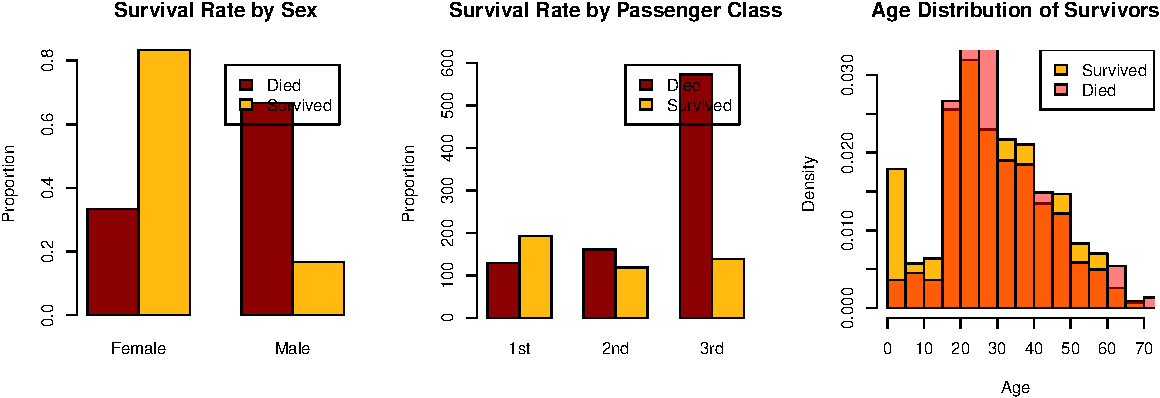
\includegraphics{ReportAssignment2_files/figure-latex/unnamed-chunk-2-1.pdf}

More males than females died, and most 3rd class passengers did not
survive. The highest number of both survivors and deaths were among
passengers aged 20 to 30.

From the below graphs we see that the majority of passengers were around
25 years old, with fewer individuals in older age groups. 1st class
passengers were generally older than those in 2nd and 3rd class.

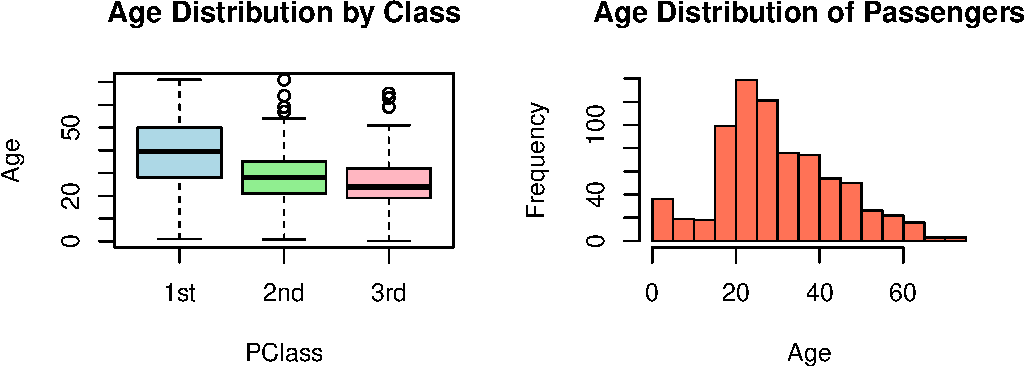
\includegraphics{ReportAssignment2_files/figure-latex/unnamed-chunk-3-1.pdf}

Let's examine how the sexes were distributed over the passenger classes.

\begin{Shaded}
\begin{Highlighting}[]
\NormalTok{sex\_class }\OtherTok{\textless{}{-}}\FunctionTok{xtabs}\NormalTok{(}\SpecialCharTok{\textasciitilde{}}\NormalTok{PClass}\SpecialCharTok{+}\NormalTok{Sex, }\AttributeTok{data=}\NormalTok{data\_titanic)}
\NormalTok{sex\_class}
\end{Highlighting}
\end{Shaded}

\begin{verbatim}
##       Sex
## PClass female male
##    1st    143  179
##    2nd    107  173
##    3rd    212  499
\end{verbatim}

As expected, since there are more males overall, each passenger class
has a higher number of males.

\begin{Shaded}
\begin{Highlighting}[]
\NormalTok{sex\_class\_surv }\OtherTok{\textless{}{-}} \FunctionTok{xtabs}\NormalTok{(Survived}\SpecialCharTok{\textasciitilde{}}\NormalTok{PClass}\SpecialCharTok{+}\NormalTok{Sex, }\AttributeTok{data=}\NormalTok{data\_titanic)}
\FunctionTok{round}\NormalTok{(sex\_class\_surv}\SpecialCharTok{/}\NormalTok{sex\_class, }\DecValTok{2}\NormalTok{)}
\end{Highlighting}
\end{Shaded}

\begin{verbatim}
##       Sex
## PClass female male
##    1st   0.94 0.33
##    2nd   0.88 0.14
##    3rd   0.38 0.12
\end{verbatim}

The survival rate decreases from 1st to 3rd class, but remains
significantly higher for females across all classes. However, the
difference in survival between females and males is less pronounced in
3rd class.

We will now fit a logistic regression model to investigate the
association between the survival status and the
predictors~\emph{PClass},~\emph{Age}~and~\emph{Sex.}

\begin{Shaded}
\begin{Highlighting}[]
\NormalTok{add\_mod }\OtherTok{\textless{}{-}} \FunctionTok{glm}\NormalTok{(Survived }\SpecialCharTok{\textasciitilde{}}\NormalTok{ PClass }\SpecialCharTok{+}\NormalTok{ Age }\SpecialCharTok{+}\NormalTok{ Sex, }\AttributeTok{data =}\NormalTok{ titanic\_clean, }\AttributeTok{family =}\NormalTok{ binomial)}
\FunctionTok{summary}\NormalTok{(add\_mod)}\SpecialCharTok{$}\NormalTok{coefficients}
\end{Highlighting}
\end{Shaded}

\begin{verbatim}
##             Estimate Std. Error z value Pr(>|z|)
## (Intercept)   3.7597    0.39757    9.46 3.18e-21
## PClass2nd    -1.2920    0.26008   -4.97 6.78e-07
## PClass3rd    -2.5214    0.27666   -9.11 7.95e-20
## Age          -0.0392    0.00762   -5.14 2.69e-07
## Sexmale      -2.6314    0.20151  -13.06 5.68e-39
\end{verbatim}

\begin{Shaded}
\begin{Highlighting}[]
\FunctionTok{cat}\NormalTok{(}\StringTok{"AIC:"}\NormalTok{, }\FunctionTok{AIC}\NormalTok{(add\_mod))}
\end{Highlighting}
\end{Shaded}

\begin{verbatim}
## AIC: 705
\end{verbatim}

The odds can be calculated using the estimates of the above table as:

\[
\text{odds} = e^{\text{log-odds}} = e^{3.7597 + (-1.292) \times \text{PClass2nd} + (-2.521) \times \text{PClass3rd} + (-0.0392) \times \text{Age} + (-2.631) \times \text{Sexmale}} 
\]

Being in 2nd or 3rd class significantly reduces the probability of
survival compared to 1st class. Older age is associated with a lower
likelihood of survival, while being male significantly decreases the
chances of survival compared to being female. The magnitude of the
coefficients reflects the sensitivity of survival odds to each variable.
Being male has the largest negative effect on survival, while age has
the smallest effect in comparison to class and sex.

\paragraph{Section b}\label{section-b}

Investigating the interaction between Age and PClass.

\begin{Shaded}
\begin{Highlighting}[]
\FunctionTok{summary}\NormalTok{(}\FunctionTok{glm}\NormalTok{(Survived}\SpecialCharTok{\textasciitilde{}}\NormalTok{Age}\SpecialCharTok{*}\NormalTok{PClass, }\AttributeTok{data=}\NormalTok{data\_titanic, }\AttributeTok{family=}\StringTok{"binomial"}\NormalTok{), }\AttributeTok{test=}\StringTok{"Chisq"}\NormalTok{)}\SpecialCharTok{$}\NormalTok{coefficients}
\end{Highlighting}
\end{Shaded}

\begin{verbatim}
##               Estimate Std. Error z value Pr(>|z|)
## (Intercept)    1.92298    0.43625   4.408 1.04e-05
## Age           -0.03584    0.00996  -3.600 3.18e-04
## PClass2nd     -0.74428    0.57155  -1.302 1.93e-01
## PClass3rd     -2.29007    0.54057  -4.236 2.27e-05
## Age:PClass2nd -0.01321    0.01587  -0.832 4.05e-01
## Age:PClass3rd  0.00464    0.01594   0.291 7.71e-01
\end{verbatim}

\begin{Shaded}
\begin{Highlighting}[]
\FunctionTok{cat}\NormalTok{(}\StringTok{"AIC:"}\NormalTok{, }\FunctionTok{AIC}\NormalTok{(}\FunctionTok{glm}\NormalTok{(Survived }\SpecialCharTok{\textasciitilde{}}\NormalTok{ Age }\SpecialCharTok{*}\NormalTok{ PClass, }\AttributeTok{data=}\NormalTok{data\_titanic, }\AttributeTok{family=}\StringTok{"binomial"}\NormalTok{)))}
\end{Highlighting}
\end{Shaded}

\begin{verbatim}
## AIC: 921
\end{verbatim}

We now investigate the interaction between Age and Sex.

\begin{Shaded}
\begin{Highlighting}[]
\FunctionTok{summary}\NormalTok{(}\FunctionTok{glm}\NormalTok{(Survived}\SpecialCharTok{\textasciitilde{}}\NormalTok{Age}\SpecialCharTok{*}\NormalTok{Sex, }\AttributeTok{data=}\NormalTok{data\_titanic, }\AttributeTok{family=}\StringTok{"binomial"}\NormalTok{), }\AttributeTok{test=}\StringTok{"Chisq"}\NormalTok{)}\SpecialCharTok{$}\NormalTok{coefficients}
\end{Highlighting}
\end{Shaded}

\begin{verbatim}
##             Estimate Std. Error z value Pr(>|z|)
## (Intercept)   0.3011     0.2990    1.01 3.14e-01
## Age           0.0294     0.0101    2.91 3.58e-03
## Sexmale      -0.5999     0.4080   -1.47 1.42e-01
## Age:Sexmale  -0.0657     0.0137   -4.80 1.57e-06
\end{verbatim}

\begin{Shaded}
\begin{Highlighting}[]
\FunctionTok{cat}\NormalTok{(}\StringTok{"AIC:"}\NormalTok{, }\FunctionTok{AIC}\NormalTok{(}\FunctionTok{glm}\NormalTok{(Survived }\SpecialCharTok{\textasciitilde{}}\NormalTok{ Age }\SpecialCharTok{*}\NormalTok{ Sex, }\AttributeTok{data=}\NormalTok{data\_titanic, }\AttributeTok{family=}\StringTok{"binomial"}\NormalTok{)))}
\end{Highlighting}
\end{Shaded}

\begin{verbatim}
## AIC: 779
\end{verbatim}

The interaction between Age and PClass does not have a significant
effect on survival. The p-values for both Age:PClass2nd (0.405) and
Age:PClass3rd (0.771) are greater than the 0.05 threshold, indicating
that these interaction terms should not be included in the final model.
The interaction between Age and Sex is statistically significant, with a
p-value of 1.57e-06 \textless{} 0.05 threshold. This suggests that the
relationship between Age and survival differs by Sex, and thus, the
interaction term should be included in the final model.

So the final model is:

\begin{Shaded}
\begin{Highlighting}[]
\NormalTok{final\_model }\OtherTok{\textless{}{-}} \FunctionTok{glm}\NormalTok{(Survived }\SpecialCharTok{\textasciitilde{}}\NormalTok{ PClass }\SpecialCharTok{+}\NormalTok{ Age}\SpecialCharTok{*}\NormalTok{Sex, }\AttributeTok{data=}\NormalTok{data\_titanic, }\AttributeTok{family=}\StringTok{"binomial"}\NormalTok{)}
\FunctionTok{summary}\NormalTok{(final\_model, }\AttributeTok{test=}\StringTok{"Chisq"}\NormalTok{)}\SpecialCharTok{$}\NormalTok{coefficients}
\end{Highlighting}
\end{Shaded}

\begin{verbatim}
##             Estimate Std. Error z value Pr(>|z|)
## (Intercept)  2.75656     0.4376   6.299 3.00e-10
## PClass2nd   -1.54337     0.2874  -5.371 7.83e-08
## PClass3rd   -2.65398     0.2914  -9.107 8.47e-20
## Age          0.00244     0.0114   0.214 8.30e-01
## Sexmale     -0.50819     0.4425  -1.148 2.51e-01
## Age:Sexmale -0.07559     0.0150  -5.036 4.74e-07
\end{verbatim}

\begin{Shaded}
\begin{Highlighting}[]
\FunctionTok{cat}\NormalTok{(}\StringTok{"AIC:"}\NormalTok{, }\FunctionTok{AIC}\NormalTok{(}\FunctionTok{glm}\NormalTok{(Survived }\SpecialCharTok{\textasciitilde{}}\NormalTok{ PClass }\SpecialCharTok{+}\NormalTok{ Age}\SpecialCharTok{*}\NormalTok{Sex, }\AttributeTok{data=}\NormalTok{data\_titanic, }\AttributeTok{family=}\StringTok{"binomial"}\NormalTok{)))}
\end{Highlighting}
\end{Shaded}

\begin{verbatim}
## AIC: 679
\end{verbatim}

This model has an AIC of 679, which is lower than the additive model's
AIC of 705. Since a lower AIC indicates a better balance between fit and
complexity, we choose this model over the additive one.

Using this model, we can now estimate the probability of survival for
each combination of levels of the factors PClass and~\emph{Sex}~for a
person of age 55.

\begin{Shaded}
\begin{Highlighting}[]
\NormalTok{new\_data }\OtherTok{\textless{}{-}} \FunctionTok{expand.grid}\NormalTok{(}\AttributeTok{Age =} \DecValTok{55}\NormalTok{, }\AttributeTok{PClass =} \FunctionTok{levels}\NormalTok{(data\_titanic}\SpecialCharTok{$}\NormalTok{PClass), }
                        \AttributeTok{Sex =} \FunctionTok{levels}\NormalTok{(data\_titanic}\SpecialCharTok{$}\NormalTok{Sex))}
\NormalTok{probabilities }\OtherTok{\textless{}{-}} \FunctionTok{predict}\NormalTok{(final\_model, }\AttributeTok{newdata =}\NormalTok{ new\_data, }\AttributeTok{type =} \StringTok{"response"}\NormalTok{)}
\FunctionTok{cbind}\NormalTok{(new\_data, }\AttributeTok{Survival\_Prob =} \FunctionTok{round}\NormalTok{(probabilities, }\DecValTok{3}\NormalTok{))}
\end{Highlighting}
\end{Shaded}

\begin{verbatim}
##   Age PClass    Sex Survival_Prob
## 1  55    1st female         0.947
## 2  55    2nd female         0.794
## 3  55    3rd female         0.559
## 4  55    1st   male         0.145
## 5  55    2nd   male         0.035
## 6  55    3rd   male         0.012
\end{verbatim}

From the table above, we see once again that being female significantly
increases the chance of survival, while survival probability decreases
progressively from 1st to 3rd class.

\paragraph{Section c}\label{section-c}

To predict survival status, we split the data into training (80\%) and
testing (20\%) subsets. We train a logistic regression model using glm()
on the training set and use predict() to generate survival probabilities
for the test set. After applying a threshold of 0.5 we classify
passengers as survived or not. The quality of the prediction can be
measured by accuracy (correct predictions/total cases) and other metrics
such as AUC-ROC and precision or recall, which provide a more detailed
evaluation, especially when dealing with class imbalance.

\paragraph{Section d}\label{section-d}

We will use Fisher's exact test to examine the effect of sex on survival
status since it is more suitable for 2x2 tables and the 2-test to
investigate the effect of class on survival status.

\begin{verbatim}
## 
##  Fisher's Exact Test for Count Data
## 
## data:  cont_table_sex
## p-value <2e-16
## alternative hypothesis: true odds ratio is not equal to 1
## 95 percent confidence interval:
##  0.0762 0.1316
## sample estimates:
## odds ratio 
##        0.1
\end{verbatim}

\begin{verbatim}
## We performed a 2-test to investigate the relationship between PClass and Survived.
\end{verbatim}

\begin{verbatim}
## Chi-squared value: 172 Degrees of freedom: 2 p-value: 3.85e-38
\end{verbatim}

Both tests show that class and sex are strongly associated with
survival.

The 2-test for the relationship between passenger class and survival
status reveals a significant association, with a test statistic of 172
and a p-value less than 2e-16. This indicates that survival is strongly
influenced by passenger class, with the null hypothesis of no
association being rejected. Similarly, Fisher's Exact Test for gender
and survival status shows a highly significant result (p-value
\textless{} 2e-16). The odds ratio of 0.1 suggests that females have
much higher odds of surviving than males, with a 95\% confidence
interval (0.0762, 0.1316) confirming that the true odds ratio is
significantly less than 1. This supports the conclusion that being
female substantially increases the chances of survival.

\paragraph{Section e}\label{section-e}

The approach in (d) is not wrong; it simply tests for associations
between categorical variables, whereas the approach in (a) and (b)
allows for adjustment of multiple factors and prediction of survival
probability.

\textbf{Logistic regression}

Advantages: Can handle both categorical and continuous predictors.
Provides odds ratios, making interpretation straightforward. Allows for
adjustment of multiple factors simultaneously. Can be used for
predicting survival probability.

Disadvantages: Assumes a linear relationship between predictor and
log-odds of the outcome. Can suffer from over-fitting if the sample size
is too small.

\textbf{2-Test}

Advantages: Simple and easy to compute even for large datasets. Works
well for categorical explanatory variables and can be applied to tables
larger than 2x2.

Disadvantages: Less accurate for small sample sizes (expected counts
\textless{} 5 can make results unreliable). Only tells you whether
dependence exists, not the nature of the dependency. Cannot be used for
prediction.

\textbf{Fisher Test}

same as the 2-test except for the following

Advantages: Accurate for small sample sizes. Provides exact p-value

Disadvantages: Can be used for tables larger than 2x2 but is
computationally expensive.

\section{Exercise 2: Military Coups}\label{exercise-2-military-coups}

\paragraph{Section a}\label{section-a-1}

Note that we transformed \emph{pollib} into a factor since we
hypothesized the effect to not be strictly linear. This was found to be
correct after comparing the different Poisson regression model outcomes.
\emph{pollib = 1} and \emph{pollib = 2} are henceforth compared to the
value of \emph{pollib = 0}.

\begin{Shaded}
\begin{Highlighting}[]
\NormalTok{poisson\_reg }\OtherTok{\textless{}{-}} \FunctionTok{glm}\NormalTok{ (miltcoup }\SpecialCharTok{\textasciitilde{}}\NormalTok{ ., }\AttributeTok{data =}\NormalTok{ data, }\AttributeTok{family =}\NormalTok{ poisson)}
\FunctionTok{summary}\NormalTok{(poisson\_reg)}
\end{Highlighting}
\end{Shaded}

\begin{verbatim}
## 
## Call:
## glm(formula = miltcoup ~ ., family = poisson, data = data)
## 
## Coefficients:
##              Estimate Std. Error z value Pr(>|z|)   
## (Intercept) -0.233427   0.997611   -0.23   0.8150   
## oligarchy    0.072566   0.035346    2.05   0.0401 * 
## pollib1     -1.103244   0.655811   -1.68   0.0925 . 
## pollib2     -1.690306   0.676650   -2.50   0.0125 * 
## parties      0.031221   0.011166    2.80   0.0052 **
## pctvote      0.015441   0.010103    1.53   0.1264   
## popn         0.010959   0.007149    1.53   0.1253   
## size        -0.000265   0.000269   -0.99   0.3244   
## numelec     -0.029619   0.069625   -0.43   0.6705   
## numregim     0.210943   0.233933    0.90   0.3672   
## ---
## Signif. codes:  0 '***' 0.001 '**' 0.01 '*' 0.05 '.' 0.1 ' ' 1
## 
## (Dispersion parameter for poisson family taken to be 1)
## 
##     Null deviance: 65.945  on 35  degrees of freedom
## Residual deviance: 28.249  on 26  degrees of freedom
## AIC: 113.1
## 
## Number of Fisher Scoring iterations: 5
\end{verbatim}

We determine that variables for which \emph{p-value \textgreater{} 0.05}
do not have a statistically significant effect on our response variable
\emph{miltcoup} which signifies the number of military coups. Moreover,
a positive coefficient details that an increase in the corresponding
variable indicates an increase in \emph{miltcoup}. We can therefore
state the following: \emph{oligarchy} and \emph{parties} are
statistically significant with a positive effect on \emph{miltcoup}.
\emph{pollib1} has a slightly significant and negative effect on
\emph{miltcoup} whilst \emph{pollib2} has a significant negative effect.
We can thus say that according to the data, countries with a higher
political liberation factor may experience less military coups.

\paragraph{Section b}\label{section-b-1}

We will now remove variables from the model one-by-one to assess which
variables are significant. For clarity we will only show the last model
and comment on which variables were removed.

At each step, we removed the variable with the largest p-value for which
\emph{p-value \textgreater{} 0.05}. This resulted in the final poisson
model with variables \emph{oligarchy}, \emph{pollib}, and
\emph{parties}. Although \emph{pollib1} has a \emph{p-value
\textgreater{} 0.05}, we include it to properly reflect the stages
within the variable.

\begin{Shaded}
\begin{Highlighting}[]
\CommentTok{\# Everything p \textless{} 0.05}
\NormalTok{poisson\_reg\_final }\OtherTok{\textless{}{-}} \FunctionTok{glm}\NormalTok{(miltcoup }\SpecialCharTok{\textasciitilde{}}\NormalTok{ oligarchy }\SpecialCharTok{+}\NormalTok{ pollib }\SpecialCharTok{+}\NormalTok{ parties, }
                    \AttributeTok{data =}\NormalTok{ data,}
                    \AttributeTok{family =}\NormalTok{ poisson)}
\FunctionTok{summary}\NormalTok{(poisson\_reg\_final)}
\end{Highlighting}
\end{Shaded}

\begin{verbatim}
## 
## Call:
## glm(formula = miltcoup ~ oligarchy + pollib + parties, family = poisson, 
##     data = data)
## 
## Coefficients:
##             Estimate Std. Error z value Pr(>|z|)    
## (Intercept)   0.2080     0.4457    0.47    0.641    
## oligarchy     0.0915     0.0226    4.05    5e-05 ***
## pollib1      -0.4954     0.4757   -1.04    0.298    
## pollib2      -1.1121     0.4595   -2.42    0.016 *  
## parties       0.0224     0.0091    2.46    0.014 *  
## ---
## Signif. codes:  0 '***' 0.001 '**' 0.01 '*' 0.05 '.' 0.1 ' ' 1
## 
## (Dispersion parameter for poisson family taken to be 1)
## 
##     Null deviance: 65.945  on 35  degrees of freedom
## Residual deviance: 32.822  on 31  degrees of freedom
## AIC: 107.6
## 
## Number of Fisher Scoring iterations: 5
\end{verbatim}

This final version of the model is in compliance with our findings for
the previously determined statistically significant variables.

\paragraph{Section c}\label{section-c-1}

We will now use the final model to make predictions about the mean
number of coups per level of liberalization. We create a hypothetical
country with mean values for the numerical variables \emph{oligarchy},
and \emph{parties}, while varying \emph{pollib} for all levels (0, 1,
and 2).

\begin{Shaded}
\begin{Highlighting}[]
\CommentTok{\# Get all columns of which to take average}
\NormalTok{selected\_vars }\OtherTok{\textless{}{-}} \FunctionTok{c}\NormalTok{(}\StringTok{"oligarchy"}\NormalTok{, }\StringTok{"parties"}\NormalTok{) }

\CommentTok{\# Compute the means}
\NormalTok{cols\_means }\OtherTok{\textless{}{-}} \FunctionTok{colMeans}\NormalTok{(data[, selected\_vars])}
\NormalTok{cols\_means}
\end{Highlighting}
\end{Shaded}

\begin{verbatim}
## oligarchy   parties 
##      5.22     17.08
\end{verbatim}

\begin{Shaded}
\begin{Highlighting}[]
\CommentTok{\# Create dataset for prediction with pollib as a factor}
\NormalTok{data2 }\OtherTok{\textless{}{-}} \FunctionTok{data.frame}\NormalTok{(}\AttributeTok{pollib =} \FunctionTok{factor}\NormalTok{(}\FunctionTok{c}\NormalTok{(}\DecValTok{0}\NormalTok{, }\DecValTok{1}\NormalTok{, }\DecValTok{2}\NormalTok{), }\AttributeTok{levels =} \FunctionTok{levels}\NormalTok{(data}\SpecialCharTok{$}\NormalTok{pollib)), }
                    \FunctionTok{t}\NormalTok{(cols\_means))}

\CommentTok{\# Make prediction}
\NormalTok{predicted\_coups }\OtherTok{\textless{}{-}} \FunctionTok{predict}\NormalTok{(poisson\_reg\_final, }\AttributeTok{newdata =}\NormalTok{ data2, }\AttributeTok{type =} \StringTok{\textquotesingle{}response\textquotesingle{}}\NormalTok{)}
\FunctionTok{data.frame}\NormalTok{(}\AttributeTok{pollib =} \FunctionTok{c}\NormalTok{(}\DecValTok{0}\NormalTok{, }\DecValTok{1}\NormalTok{, }\DecValTok{2}\NormalTok{), }\AttributeTok{predicted\_coups =}\NormalTok{ predicted\_coups)}
\end{Highlighting}
\end{Shaded}

\begin{verbatim}
##   pollib predicted_coups
## 1      0           2.908
## 2      1           1.772
## 3      2           0.956
\end{verbatim}

From this we find the mean for \emph{oligarchy} to be \emph{5.222} and
the mean for \emph{parties} to be \emph{17.083}. Furthermore we find the
number of predicted coups to decrease as the index for political
liberalization increases. We find that our hypothetical country with no
political liberalization experiences roughly \emph{2.91} military coups,
with limited rights it experiences an estimated \emph{1.77} coups and
under full political liberalization it is estimated to expect roughly
\emph{0.96} military coups. These results indicate that greater
political liberalization is associated with fewer military coups.

\section{Exercise 3: Stormer
viscometer}\label{exercise-3-stormer-viscometer}

\paragraph{Section a}\label{section-a-2}

To understand the relationships between the variables, a scatterplot of
the data is plotted below:

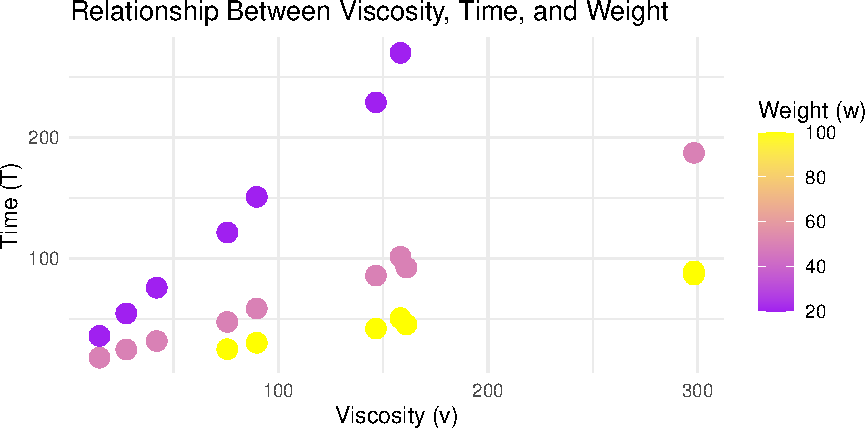
\includegraphics{ReportAssignment2_files/figure-latex/unnamed-chunk-20-1.pdf}

The scatterplot visualizes that higher weight values correspond to lower
time values, demonstrating an inverse relationship between weight and
time. Additionally, the pattern of points suggests a nonlinear
relationship between viscosity and time, supporting the theoretical
nonlinear model:

\[ 
T = \frac{\theta_1 v}{w - \theta_2} + e
\] However, in order to estimate the parameters \(\theta_1\) and
\(\theta_2\), since the theoretical model can be rewritten to a linear
form, we can first apply linear regression to obtain initial estimates
using the following formula: \[
wT = \theta_1 v + \theta_2 T + (w - \theta_2)e
\] As the variance of the error term is not constant, we have to take
into account heteroscedasticity. For this, the variance of \(wT\)
becomes the following: \[
Var(wT) = \sigma^2(w - \theta_2)^2
\] We use Weighted Least Squares and set the weights in the regression
as, using an initial guess for \(\theta_2\) to do the linear regression:
\[
w_i = \frac{1}{(w_i - \hat{\theta}_2)^2}
\]

\begin{Shaded}
\begin{Highlighting}[]
\NormalTok{theta2\_init }\OtherTok{=} \FunctionTok{mean}\NormalTok{(stormer}\SpecialCharTok{$}\NormalTok{Wt)}
\NormalTok{weights\_wls }\OtherTok{=} \DecValTok{1} \SpecialCharTok{/}\NormalTok{ (stormer}\SpecialCharTok{$}\NormalTok{Wt }\SpecialCharTok{{-}}\NormalTok{ theta2\_init)}\SpecialCharTok{\^{}}\DecValTok{2}
\NormalTok{linear\_model\_wls }\OtherTok{=} \FunctionTok{lm}\NormalTok{(Wt }\SpecialCharTok{*}\NormalTok{ Time }\SpecialCharTok{\textasciitilde{}}\NormalTok{ Viscosity }\SpecialCharTok{+}\NormalTok{ Time, }\AttributeTok{data =}\NormalTok{ stormer, }\AttributeTok{weights =}\NormalTok{ weights\_wls)}
\FunctionTok{summary}\NormalTok{(linear\_model\_wls)}
\end{Highlighting}
\end{Shaded}

\begin{verbatim}
## 
## Call:
## lm(formula = Wt * Time ~ Viscosity + Time, data = stormer, weights = weights_wls)
## 
## Weighted Residuals:
##    Min     1Q Median     3Q    Max 
## -58.56 -10.64  -2.31   7.60  44.11 
## 
## Coefficients:
##             Estimate Std. Error t value Pr(>|t|)    
## (Intercept)   222.57      79.26    2.81    0.011 *  
## Viscosity      26.50       1.69   15.64  1.1e-12 ***
## Time            5.15       2.77    1.86    0.078 .  
## ---
## Signif. codes:  0 '***' 0.001 '**' 0.01 '*' 0.05 '.' 0.1 ' ' 1
## 
## Residual standard error: 23 on 20 degrees of freedom
## Multiple R-squared:  0.993,  Adjusted R-squared:  0.993 
## F-statistic: 1.47e+03 on 2 and 20 DF,  p-value: <2e-16
\end{verbatim}

The found estimated values are \(\theta_1 = 26.499\) and
\(\theta_2 = 5.150\), where only the value of \(\theta_1\) is
statistically significant. Using these estimated values, we can do
nonlinear regression:

\begin{Shaded}
\begin{Highlighting}[]
\NormalTok{theta1\_wls }\OtherTok{\textless{}{-}} \FunctionTok{coef}\NormalTok{(linear\_model\_wls)[}\StringTok{"Viscosity"}\NormalTok{]}
\NormalTok{theta2\_wls }\OtherTok{\textless{}{-}} \FunctionTok{coef}\NormalTok{(linear\_model\_wls)[}\StringTok{"Time"}\NormalTok{]}
\NormalTok{nls\_model\_weighted }\OtherTok{\textless{}{-}} \FunctionTok{nls}\NormalTok{(Time }\SpecialCharTok{\textasciitilde{}}\NormalTok{ (theta1 }\SpecialCharTok{*}\NormalTok{ Viscosity) }\SpecialCharTok{/}\NormalTok{ (Wt }\SpecialCharTok{{-}}\NormalTok{ theta2), }
                          \AttributeTok{data =}\NormalTok{ stormer,}
                          \AttributeTok{start =} \FunctionTok{list}\NormalTok{(}\AttributeTok{theta1 =}\NormalTok{ theta1\_wls, }\AttributeTok{theta2 =}\NormalTok{ theta2\_wls),}
                          \AttributeTok{weights =} \DecValTok{1} \SpecialCharTok{/}\NormalTok{ (Wt }\SpecialCharTok{{-}}\NormalTok{ theta2\_wls)}\SpecialCharTok{\^{}}\DecValTok{2}\NormalTok{)}

\FunctionTok{summary}\NormalTok{(nls\_model\_weighted)}
\end{Highlighting}
\end{Shaded}

\begin{verbatim}
## 
## Formula: Time ~ (theta1 * Viscosity)/(Wt - theta2)
## 
## Parameters:
##        Estimate Std. Error t value Pr(>|t|)    
## theta1    29.64       2.62   11.29  2.2e-10 ***
## theta2     2.06       1.62    1.27     0.22    
## ---
## Signif. codes:  0 '***' 0.001 '**' 0.01 '*' 0.05 '.' 0.1 ' ' 1
## 
## Residual standard error: 0.342 on 21 degrees of freedom
## 
## Number of iterations to convergence: 3 
## Achieved convergence tolerance: 2.11e-06
\end{verbatim}

The final estimated values are \(\theta_1 = 29.637\) and
\(\theta_2 = 2.065\), where only \(\theta_1\) seems statistically
significant. Additionally, the residual standard error is smaller
(0.342) compared to the linear model (22.96) indicating that this model
has much less unexplained variation.

\begin{verbatim}
## Warning: Using `size` aesthetic for lines was deprecated in ggplot2 3.4.0.
## i Please use `linewidth` instead.
## This warning is displayed once every 8 hours.
## Call `lifecycle::last_lifecycle_warnings()` to see where this warning was
## generated.
\end{verbatim}

\begin{verbatim}
## Warning: Removed 41 rows containing missing values or values outside the scale range
## (`geom_line()`).
\end{verbatim}

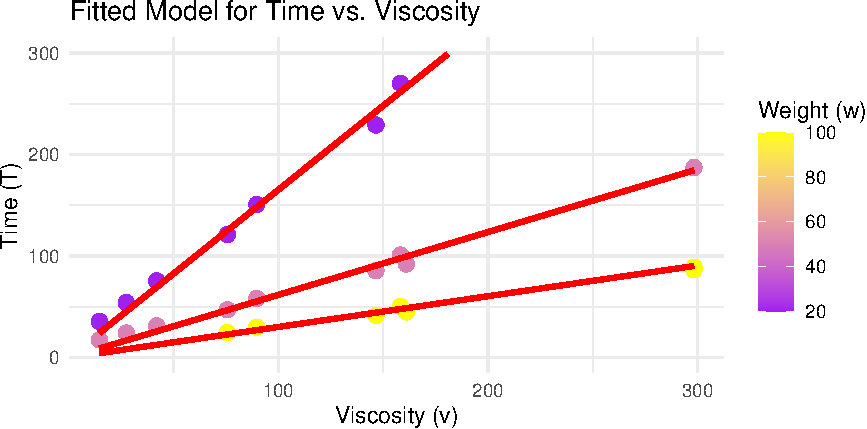
\includegraphics{ReportAssignment2_files/figure-latex/unnamed-chunk-23-1.pdf}

The final plot shows that the nonlinear regression model fits the data
well, capturing the expected trend between viscosity and time while
accounting for different weight values. The fitted curves align closely
with the data points, confirming that the nonlinear model is more
appropriate than a linear model.However, the separation of curves
suggests some variation in the effect of weight, and \(\theta_2\) was
not statistically significant, indicating potential refinements in the
model.

\paragraph{Section b}\label{section-b-2}

A two-tailed t-test is conducted, as we have no expectation about
whether \(\theta_1\) will be greater or smaller than 25; it could differ
in either direction. We consider the null hypothesis H0: \(\theta_1\) =
25. For the test, we use the estimated \(\theta_1\) and its standard
error obtained from question a). The test resulted in a t-statistic of
4.81 and a p-value of 9.45e-05, which is far below the typical
significance level of 0.05. This means we reject H0 and conclude that
\(\theta_1\) is significantly different from 25, further supporting the
nonlinear model's results.

\begin{Shaded}
\begin{Highlighting}[]
\NormalTok{theta1\_hat }\OtherTok{=} \FloatTok{29.4013}  \CommentTok{\# Estimated parameter}
\NormalTok{theta1\_se }\OtherTok{=} \FloatTok{0.9155}    \CommentTok{\# Standard error}
\NormalTok{theta1\_h0 }\OtherTok{=} \DecValTok{25}        \CommentTok{\# Hypothesized value under H0}
\NormalTok{df }\OtherTok{=} \DecValTok{21}               \CommentTok{\# Degrees of freedom from nls summary}

\NormalTok{t\_stat }\OtherTok{=}\NormalTok{ (theta1\_hat }\SpecialCharTok{{-}}\NormalTok{ theta1\_h0) }\SpecialCharTok{/}\NormalTok{ theta1\_se}
\NormalTok{p\_value }\OtherTok{=} \DecValTok{2} \SpecialCharTok{*} \FunctionTok{pt}\NormalTok{(}\SpecialCharTok{{-}}\FunctionTok{abs}\NormalTok{(t\_stat), df)}
\end{Highlighting}
\end{Shaded}

\textbf{Test Statistic (t):} 4.81

\textbf{P-value:} 9.454e-05

\paragraph{Section c}\label{section-c-2}

For computing the 92\% confidence interval for \(\theta_1\) and
\(\theta_2\), we consider the following formula to calculate the
z-value: \[
\hat{\theta} \pm z_{\alpha/2} \cdot SE(\theta)
\] where \(z_{\alpha/2}\) is the critical value from the standard normal
distribution. For a 92\% confidence level, the significance level is
\(\alpha\) = 0.08, thus: \[z_{0.04/2} = z_{0.02} \approx 1.75\]

This gave a 92\% CI for \(\theta_1\)\hspace{0pt} of {[}27.80, 31.00{]}
and for \(\theta_2\)\hspace{0pt} of {[}1.05, 3.38{]}, meaning we are
92\% confident that the true values lie within these intervals. Since
the confidence interval for \(\theta_1\)\hspace{0pt} does not include
25, it further supports rejecting H0\hspace{0pt} from question b).

\begin{Shaded}
\begin{Highlighting}[]
\NormalTok{theta1\_hat }\OtherTok{\textless{}{-}} \FloatTok{29.4013}  \CommentTok{\# Estimated θ1}
\NormalTok{theta1\_se }\OtherTok{\textless{}{-}} \FloatTok{0.9155}    \CommentTok{\# Standard error of θ1}
\NormalTok{theta2\_hat }\OtherTok{\textless{}{-}} \FloatTok{2.2183}   \CommentTok{\# Estimated θ2}
\NormalTok{theta2\_se }\OtherTok{\textless{}{-}} \FloatTok{0.6655}    \CommentTok{\# Standard error of θ2}

\NormalTok{z\_value }\OtherTok{=} \FunctionTok{qnorm}\NormalTok{(}\FloatTok{0.96}\NormalTok{)  }\CommentTok{\# 1.75}

\NormalTok{theta1\_CI }\OtherTok{=} \FunctionTok{c}\NormalTok{(theta1\_hat }\SpecialCharTok{{-}}\NormalTok{ z\_value }\SpecialCharTok{*}\NormalTok{ theta1\_se, theta1\_hat }\SpecialCharTok{+}\NormalTok{ z\_value }\SpecialCharTok{*}\NormalTok{ theta1\_se)}
\NormalTok{theta2\_CI }\OtherTok{=} \FunctionTok{c}\NormalTok{(theta2\_hat }\SpecialCharTok{{-}}\NormalTok{ z\_value }\SpecialCharTok{*}\NormalTok{ theta2\_se, theta2\_hat }\SpecialCharTok{+}\NormalTok{ z\_value }\SpecialCharTok{*}\NormalTok{ theta2\_se)}
\end{Highlighting}
\end{Shaded}

\textbf{92\% CI for θ1:} {[} 27.8 31 {]}

\textbf{92\% CI for θ2:} {[} 1.05 3.38 {]}

\paragraph{Section d}\label{section-d-1}

The expected values are computed using the nonlinear model with \(w\) =
50, and viscosity values ranging from 10 to 300. The 94\% confidence
intervals were derived using asymptotic normality, where the standard
error of T was estimated through error propagation. The confidence
bounds were calculated as:

\[T(v) \pm z_{\alpha/2} \cdot SE(T)\]

where \(z_{0.03}\) = 1.88 is the critical value for a 94\% confidence
level. The plot shows the expected T along with a shaded confidence
band, indicating the uncertainty in our estimates. The confidence
interval widens as viscosity increases, reflecting greater uncertainty
for larger \(v\). The linear trend suggests a strong relationship
between viscosity and time, but further diagnostics are needed to
confirm model assumptions. Overall, the plot aligns well with the
theoretical nonlinear model, supporting its validity over a simple
linear approximation.

\begin{verbatim}
\end{verbatim}

\begin{Shaded}
\begin{Highlighting}[]
\NormalTok{theta1\_hat }\OtherTok{=} \FloatTok{29.4013}  \CommentTok{\# Estimate of theta1}
\NormalTok{theta2\_hat }\OtherTok{=} \FloatTok{2.2183}   \CommentTok{\# Estimate of theta2}
\NormalTok{theta1\_se }\OtherTok{=} \FloatTok{0.9155}    \CommentTok{\# Standard error of theta1}
\NormalTok{theta2\_se }\OtherTok{=} \FloatTok{0.6655}    \CommentTok{\# Standard error of theta2}
\NormalTok{w\_fixed }\OtherTok{=} \DecValTok{50}
\NormalTok{v\_values }\OtherTok{=} \FunctionTok{seq}\NormalTok{(}\DecValTok{10}\NormalTok{, }\DecValTok{300}\NormalTok{, }\AttributeTok{length.out =} \DecValTok{100}\NormalTok{)}

\NormalTok{T\_hat }\OtherTok{=}\NormalTok{ (theta1\_hat }\SpecialCharTok{*}\NormalTok{ v\_values) }\SpecialCharTok{/}\NormalTok{ (w\_fixed }\SpecialCharTok{{-}}\NormalTok{ theta2\_hat)}
\NormalTok{T\_se }\OtherTok{=} \FunctionTok{sqrt}\NormalTok{(}
\NormalTok{  (v\_values }\SpecialCharTok{/}\NormalTok{ (w\_fixed }\SpecialCharTok{{-}}\NormalTok{ theta2\_hat))}\SpecialCharTok{\^{}}\DecValTok{2} \SpecialCharTok{*}\NormalTok{ theta1\_se}\SpecialCharTok{\^{}}\DecValTok{2} \SpecialCharTok{+}
\NormalTok{  (theta1\_hat }\SpecialCharTok{*}\NormalTok{ v\_values }\SpecialCharTok{/}\NormalTok{ (w\_fixed }\SpecialCharTok{{-}}\NormalTok{ theta2\_hat)}\SpecialCharTok{\^{}}\DecValTok{2}\NormalTok{)}\SpecialCharTok{\^{}}\DecValTok{2} \SpecialCharTok{*}\NormalTok{ theta2\_se}\SpecialCharTok{\^{}}\DecValTok{2}
\NormalTok{)}

\NormalTok{z\_value }\OtherTok{=} \FunctionTok{qnorm}\NormalTok{(}\FloatTok{0.97}\NormalTok{)}
\NormalTok{T\_lower }\OtherTok{=}\NormalTok{ T\_hat }\SpecialCharTok{{-}}\NormalTok{ z\_value }\SpecialCharTok{*}\NormalTok{ T\_se}
\NormalTok{T\_upper }\OtherTok{=}\NormalTok{ T\_hat }\SpecialCharTok{+}\NormalTok{ z\_value }\SpecialCharTok{*}\NormalTok{ T\_se}
\end{Highlighting}
\end{Shaded}

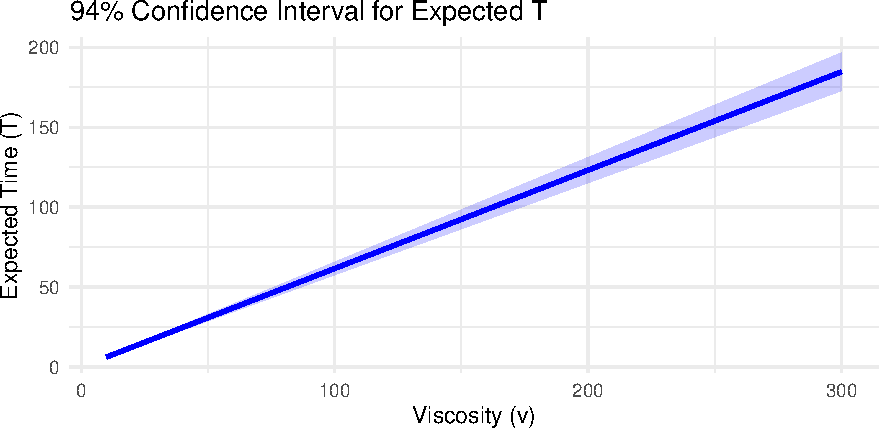
\includegraphics{ReportAssignment2_files/figure-latex/unnamed-chunk-29-1.pdf}

\paragraph{Section e}\label{section-e-1}

To investigate whether the smaller model with \(\theta_1\) = 25 is
appropriate, we compare it to the estimated model using hypothesis
testing and model evaluation metrics. From question b), the T-test
rejected H0: \(\theta_1\) =25 with a p-value of 9.45e-05, indicating
that setting \(\theta_1\) = 25 significantly deviates from the data.
Additionally, the 92\% confidence interval for \(\theta_1\) of {[}27.80,
31.00{]} does not contain 25, further supporting that the restriction is
inappropriate. A likelihood ratio test could be performed to formally
compare the smaller model to the unrestricted model, however, the
hypothesis test already suggests a poor fit. Constraining \(\theta_1\)
may lead to higher residual errors and reduced model flexibility, making
the model less accurate. Given these findings, the smaller model does
not seem appropriate, as it forces an assumption that contradicts the
observed data. Therefore, the unrestricted nonlinear model remains the
more valid choice.

\end{document}
